\section{Introduction}

% What is the problem?
File system metadata services in HPC have scalability problems. It has been
shown that HPC workloads, especially checkpoint-restart jobs, are resource
intensive primarily due to contention for the same directories and inodes ({\it
e.g.}, path traversal). Applications perform better with dedicated metadata
servers~\cite{sevilla:sc15-mantle, ren:sc2014-indexfs} but provisioning a
metadata server for every client is unreasonable. This problem is exacerbated
by current trends in HPC, where architectures are transitioning from complex
storage stacks with burst buffer, file system, object store, and tape tiers to
more simplified stackis with just a burst buffer and object
store~\cite{bent:login16-hpc-trends}; this puts more pressure on data access
instead of data movement.

% What is HPC doing?
HPC's unique requirements for file systems ({\it e.g.}, fast creates) and well
defined workloads ({\it e.g.}, workflows) have given rise to file systems with
weaker consistency constraints than POSIX and less durability than programmers
are accustomed to.  Without these constraints, HPC systems can do more
client side processing with an emphasis on serverless metadata services.

One popular approach for relaxing consistency and durability is to ``decouple
the namespace", where clients lock the subtree they want exclusive access to so
other clients cannot interfere. This delayed merge ({\it i.e.} a form of
eventual consistency) and relaxed durability improves performance and
scalability by avoiding the costs of RPCs, synchronization, false sharing, and
serialization.  While the performance benefits are obvious for these users,
applications that rely on stronger consistency or durability guarantees must be
re-written or deployed on a different system. The consistency and durability
semantics for these systems is shown in Table~\ref{table:namespaces}.

\begin{figure}[tb]
\centering
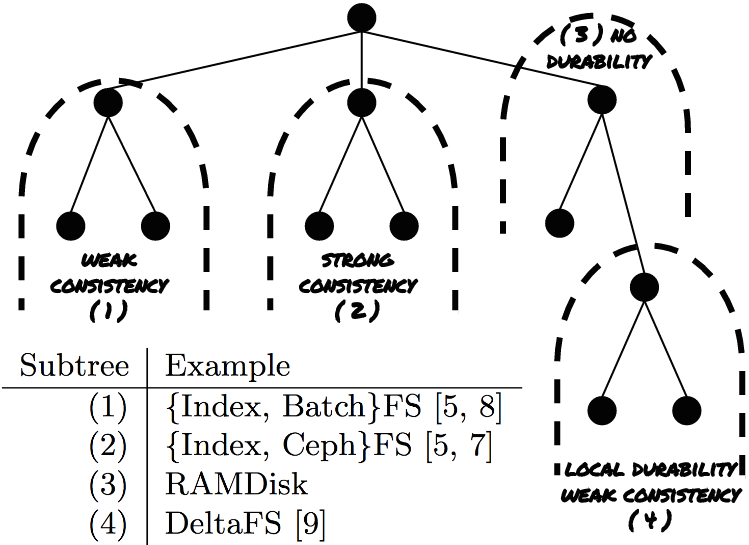
\includegraphics[width=75mm]{figures/subtree-policies.png}
\caption{Administrators can assign consistency and durability policies to
subtrees to get the benefits of some of the state-of-the-art HPC architectures.
}\label{fig:subtree-policies}
\end{figure}

\begin{table}
\begin{tabular}{ r | l | l }
              & Decoupled & Global    \\
              & Namespace & Namespace \\\hline
  Example     & BatchFS~\cite{zheng:pdsw2014-batchfs} & CephFS~\cite{weil:sc2004-dyn-metadata} \\
              & DeltaFS~\cite{zheng:pdsw2015-deltafs} & IndexFS~\cite{ren:sc2014-indexfs}      \\
  Consistency & eventual & strong     \\
  Durability  & node local & global  \\
\end{tabular}
\caption{State-of-the-art systems in HPC improve file system metadata
performance by relaxing consistency and durability
guarantees.\label{table:namespaces}}
\end{table}

% What did we do
We propose subtree policies, an interface that lets future programmers control
how the storage system manages different parts of the file system namespace.  For performance one
subtree can adopt weaker consistency semantics while another subtree can retain
the rigidity of POSIX's strong consistency. Figure~\ref{fig:subtree-policies}
shows an example setup where a single global namespace has directories for
applications designed for different, state-of-the-art HPC architectures.  We
present Cudele, a prototype programmable file system that supports different
degrees of consistency and durability by exposing mechanisms used within the
file system as a client library.  Cudele supports 3 forms of consistency
(invisible, eventual, and strong) and 3 degrees of durability (none, local, and
global) giving the administrator a wide range of policies and optimizations
that can be custom fit to an application. Our contributions: 

\begin{enumerate}

  \item a prototype that lets administrators program a range of
  consistency and durability semantics (9 permutations), allowing them to custom
  fit the storage system to the application.

  \item an API for programming consistency/durability policies and assigning
  them to subtrees in the file system namespace.

  \item a comparison of the strategies used in recently proposed research systems against
  previously unexplored metadata designs.

\end{enumerate}

% Results
Our results confirm the assertions of ``clean-state" research systems that
decouple namespaces; specifically that the technique drastically improve
performance (104\(\times\) speed up) but we go a step further by quantifying
the costs of merging updates (7\(\times\) slow down) and maintaining durability
(\(10\times\) slow down). We also show the effect of having a metadata specific
file format in systems that are based on in-memory data structures.
Section~\ref{sec:related-work} places Cudele in the context of other related
work. Section~\ref{sec:posix-overheads} quantifies the cost of POSIX
consistency and system-defined durability and
Section~\ref{sec:methodology-decoupled-namespaces} presents the Cudele
prototype and API. Section~\ref{sec:implementation} describes Cudele's
mechanisms and shows how re-using internal subsystems results in an
implementation of less than 500 lines of code. The evaluation in
Section~\ref{sec:evaluation} quantifies the overheads and performance gains of
explored and previously unexplored metadata designs.

